\subsection{Block Diagram}

YAPPL (it is appropriate to shout when pronouncing the all-caps name) is implemented using a standard model for compilers. The input is tokenized, parsed, and then translated into OCaml. The components are implemented in ocamllex, ocamlyacc and OCaml. The generated .ml can then be compiled into executable code.  \texttt{yapplc} automates this process.\\
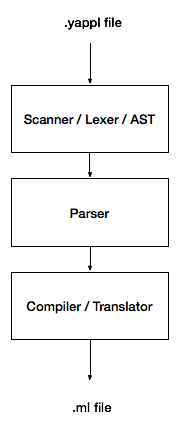
\includegraphics[width=1.5in]{block-diagram.png}

\subsection{Components}
\subsubsection{Symbol Table}
The translator builds an initial table for storing user specified identifiers and their type. The table can also point to a parent table, allowing for scoping. This scoping occurs, for example, in a declaration of a \term{(} \nterm{pattern} \term{::} \nterm{pattern} \term{)} match. To detect a problematic pattern such as  \term{(a::a)}, the first \term{a} is added to a blank symbol subtable. When converting the second \term{a} into output, the compiler will notice that an \term{a} has already been created in the subtable and raise an error. 
\subsubsection{expr\_to\_string} 
This is the main function for the evaluation of the program expression and returns both a string representation of the parse tree it is given, and its type. It is called recursively to evaluate the program parse tree. As part of the output generation, types are checked for validity. When the function converts identifiers to strings, it will first check if that identifier is built-in, such as \texttt{print}, before performing a lookup with the symbol table.
\subsubsection{Memoization}
Memoization is implemented using a hash table that is populated when a memoized function is called with a new parameter.  In the generated code, all user-defined identifiers (not just those in the memoized function) will be prepended with \texttt{yappl\_}, to prevent namespace collisions with OCaml identifiers, such as hash tables, used by the YAPPL compiler.
\subsubsection{Compiling to executable}
The \texttt{ocamlc} utility links the compiled generated code with built-in OCaml functionality such as \texttt{rand}. It also prepends \texttt{stdlib.ypl}, if it exists, to function as a standard library.